%% LaTeX2e class for student theses
%% sections/evaluation.tex
%% 
%% Karlsruhe Institute of Technology
%% Institute for Program Structures and Data Organization
%% Chair for Software Design and Quality (SDQ)
%%
%% Dr.-Ing. Erik Burger
%% burger@kit.edu
%%
%% Version 1.3.6, 2022-09-28

\chapter{Related Work}
\label{ch:Related_work}
We present related work for this thesis in this chapter. First, we will outline the basic idea of each active learning strategy we
use in our experiments. Next, we give an overview of the continual learning approaches we use. Finally, we will introduce ActiveThief, the
model stealing framework we extend in this thesis.


\section{Active Learning}
\label{sec:Related_work:Active_Learning}
In this section, we will present the active learning strategies we will use in our experiments. These are least confidence
(\gls{lc}), CoreSet, bayesian active learning by disagreement (\gls{bald}), batch active learning by diverse gradient embeddings (\gls{badge}), and 
variational adversarial active learning (\gls{vaal}). While we aim to give a detailed explanation of these approaches, we refer to the
original papers for any further details. \par

\subsection{Least Confidence}
\label{sec:Related_work:Active_Learning:Least_Confidence}
Least confidence (\gls{lc}) is one of the earlier approaches to active learning. \gls{lc} is an uncertainty-based active learning
approach proposed by Lewis et al. \cite{lewis1995sequential} in 1994. The idea behind \gls{lc} is that the next points to label should be the 
ones with the lowest prediction probability. More formally, the data queried will be the following:
\begin{equation}
    \argmin_{x \in U} \max_{y \in Y} p(y|x)
\end{equation}
where $U$ is the set of unlabeled data points and $Y$ is the set of possible labels. \par

\subsection{CoreSet}
\label{sec:Related_work:Active_Learning:CoreSet}
CoreSet, sometimes named $k$-center strategy, is an active learning method specifically proposed for \glspl{cnn} \cite{sener2017active}.
Sener and Savarese redefine the pool-based active learning problem (for the original definition, see 
section \ref{sec:PoolBasedActiveLearning}) as 
\begin{equation}
    \min_{s^1 \subseteq U: |s^1| \leq b } \abs{\frac{1}{|L \cup U|} \sum_{x_i,y_i \in L \cup U} \mathcal{L}(x_i,y_i;L \cup s^1) - \frac{1}{|L \cup s^1|} 
    \sum_{j \in L \cup s^1} \mathcal{L}(x_j,y_j,L \cup s^1)}, 
\end{equation}
where $L$ is the labeled set, $U$ is the unlabeled set and $b$ is the batch size.
Informally, we select the data points to add to the labeled pool, which ensure the best loss approximation
of a model trained on the labeled set compared to a model trained on the whole dataset. The authors assume zero training error, which
simplifies the equation above to
\begin{equation}
    \frac{1}{|L \cup U|} \sum_{x_i,y_i \in L \cup U} \mathcal{L}(x_i,y_i;L \cup s^1)
\end{equation}
Sener and Savarese show that minimizing this equation is equivalent to solving the $k$-Center problem \cite{wolf2011facility}, i.e.
\begin{equation}
    \min_{s^1: |s^1| \leq b} \max_i \min_{j \in s^1 \cup L}  \Delta (x_i,x_j)
\end{equation}
This problem is NP-hard but can be solved by the 2-OPT greedy algorithm presented in algorithm \ref{alg:kCenterGreedy}.
\begin{algorithm}
    \caption{$k$-Center-Greedy} \label{alg:kCenterGreedy}
    \begin{algorithmic}
        \Require data $x_i$, labeled pool $L$ and budget $b$
        \State Initialize s = $L$
        \Repeat
        \State $u = \argmax_{x_i \in U \setminus s} \min_{x_j \in s} \Delta(x_i,x_j)$
        \State $s = s \cup \{u\}$
        \Until{$|s| = b$}
        \return $s \setminus L$
    \end{algorithmic}
\end{algorithm}
The authors propose a more sophisticated algorithm that performs marginally better than the greedy solution but is approximately 
four times slower. Therefore, we omit the proposed algorithm in this section.

\subsection{Bayesian Active Learning by Disagreement}
\label{sec:Related_work:Active_Learning:BALD}
Bayesian active learning by disagreement (\gls{bald}) is an uncertainty-based active learning strategy proposed by Houlsby et al. 
\cite{houlsby2011bayesian}. \gls{bald} uses Shannon's entropy \cite{cover1991information} to determine a model's prediction uncertainty for a given
unlabeled data point. More precisely, a learner using \gls{bald} will query the sample(s) fulfilling the following condition
\begin{equation}
    \argmax_{x \in U} H[y \mid x, L] - \mathbb{E}_{\theta \sim p(\theta \mid L)} [H[y \mid x, \theta]]
\end{equation}
where $H$ is the entropy, $U$ is the set of unlabeled data points, and $L$ is the set of labeled data points.
Informally, \gls{bald} selects those data points with the largest gap between the model's actual prediction uncertainty and the model's expected
prediction uncertainty. Since the expected prediction uncertainty cannot be computed given that the parameter distribution conditioned on the
previously observed data is unknown, \gls{bald} uses Monte Carlo sampling to approximate the expected prediction uncertainty. For neural networks, Monte
Carlo dropout \cite{gal2016dropout} can be applied.

\subsection{Batch Active Learning by Diverse Gradient Embeddings}
\label{sec:Related_work:Active_Learning:BADGE}
Batch active learning by diverse gradient embeddings (\gls{badge}) \cite{ash2019deep} is a batch active learning strategy that combines both model uncertainty
and batch diversity to select the next batch of data points to label. The authors were inspired to develop \gls{badge} by the observation that diversity-based
active learning strategies perform well in the first few iterations, while uncertainty-based approaches perform well in the later stages of active learning.
\gls{badge} therefore incorporates both uncertainty and diversity in its selection strategy. Furthermore, \gls{badge} uses the
gradient with respect to the output layer as a measure of model uncertainty, similar to the ideas of Zhang et al. \cite{zhang2017active} and Settles et al. \cite{settles2007multiple}.
Since \gls{badge} works on unlabeled data points, the gradient cannot be computed analytically because the label is unknown. Therefore, \gls{badge} uses the hypothetical
label $\hat{y}(x)$ as a proxy for the true label and computes the gradient of the cross-entropy loss on the hypothetical label as an approximation of the
actual gradient. To incorporate diversity, \gls{badge} uses $k$-means++ initialization \cite{arthur2007k} for the gradient embeddings to sample the next batch of data
points to label. The authors demonstrate \gls{badge}'s agnosticism towards model architecture, training hyperparameters, and datasets in mutliple experiments.
\begin{algorithm}
    \caption{\gls{badge}} \label{alg:Badge}
    \begin{algorithmic}[1]
        \Require Neural network $f(x;\theta)$, unlabeled pool $U$, labeled pool $L=\emptyset$, number of iterations $T$, bath size $b$
        \State Labeled dataset $L \leftarrow k$ random samples from $U$ together with their labels
        \State Train initial model $\theta_1$ on $L$
        \For{$t = 1,2,\ldots,T$}
            \State For all examples $x$ in $U \setminus L$:
            \begin{enumerate}[leftmargin=0.8in]
                \item Compute its hypothetical label $\hat{y}(x) = h_{\theta_t}(x)$
                \item Compute gradient embeddings $g_x = \frac{\partial}{\partial \theta_{out}} \mathcal{L}_{\text{CE}}(f(x;\theta_t),\hat{y}(x))$, where
                $\theta_{out}$ refers to parameters of the final (output) layer.
            \end{enumerate}
            \State Compute $S_t$, a subset of $U \setminus L$ of size $b$, using the $k$-MEANS++ seeding algorithm on {\color{white} 123}$\{ g_x: x \in U
            \setminus L\}$ and query for their labels.
            \State Update labeled pool $L \leftarrow L \cup S_t$
            \State Train new model $\theta_{t+1}$ on $L$
        \EndFor
        \return Final model $\theta_T$
    \end{algorithmic}
\end{algorithm}

\subsection{Variational Adversarial Active Learning}
\label{sec:Related_work:Active_Learning:VAAL}
Variational adversarial active learning (\gls{vaal}) is a representation-based active learning strategy proposed by Sinha et al. \cite{sinha2019variational}. 
\gls{vaal} uses a $\beta$-variational autoencoder (\gls{vae}) \cite{higgins2017beta} and a discriminator to select the most informative samples to query.
Thereby, the encoder learns a low-dimensional space for the distribution of the labeled and the unlabeled data reconstructed by the decoder. 
The discriminator is trained to distinguish between the labeled and the unlabeled data and given the encoder's latent representation of a data point as an
input. We provide a visual summary of the approach in figure \ref{fig:VAAL}. \par
More formally, the encoder learns the distribution of $X_U$ and $X_L$ where $X_U$ is the unlabeled pool and $(X_L, Y_L)$ is the labeled pool. The encoder
aims to minimize the \gls{kl} divergence \cite{goldberger2004hierarchical} between the reconstructed distribution $q_\Phi (z_L | x_L)$ and
the real distribution $p(z)$ of the labeled data, which we assume to be a unit Gaussian. Simultaneously, the encoder aims to minimize the \gls{kl} divergence
between $q_\Phi (z_U | x_U)$ and $p(z)$. This results in the following objective function for the \gls{vae}:
\begin{equation}
    \mathcal{L}^{trd}_{VAE} = \mathbb{E}[\log p_\theta (x_L | z_L)] - \beta D_{KL} (q_\Phi (z_L | x_L) || p(z)) + \mathbb{E}[\log p_\theta (x_U | z_U)] - \beta D_{KL} (q_\Phi (z_U | x_U) || p(z))
\end{equation}
where $p_\theta$ and $q_\Phi$ are the decoder and the encoder. The discriminator $D$ is trained to distinguish between the latent space representation
of labeled and unlabeled data. Additionally, the \gls{vae} is trained to make samples from the labeled and
unlabeled data indistinguishable to complicate the classification of the discriminator. The adversarial objective function for the discriminator is given by:
\begin{equation}
    \mathcal{L}^{adv}_{VAE} = - \mathbb{E}[\log(D(q_\theta (z_L | x_L)))] - \mathbb{E}[\log(D(q_\theta(z_U | x_U)))].
\end{equation}
Both equations above result in the following final loss function for the \gls{vae}:
\begin{equation}
    \mathcal{L}_{VAE} = \lambda_1 \mathcal{L}^{trd}_{VAE} + \lambda_2 \mathcal{L}^{adv}_{VAE}
\end{equation}
where $\lambda_1$ and $\lambda_2$ are hyperparameters, trading off between adversarial training and optimal reconstruction. \par
The discriminator loss is given by:
\begin{equation}
    \mathcal{L}_D = - \mathbb{E}[\log(D(q_\theta (z_L | x_L)))] - \mathbb{E}[\log (1- D(q_\theta (z_U | x_U)))].
\end{equation}
To query a batch of samples of size $b$, the \gls{vae} and discriminator are first trained on the entire pool of labeled and unlabeled data for a
pre-specified number of epochs $e$. The samples chosen by \gls{vaal} are the ones where the discriminator is most confident about their belonging to the unlabeled
pool or, in other words, least confident about their belonging to the labeled pool.
\begin{figure} [ht]
    \centering
    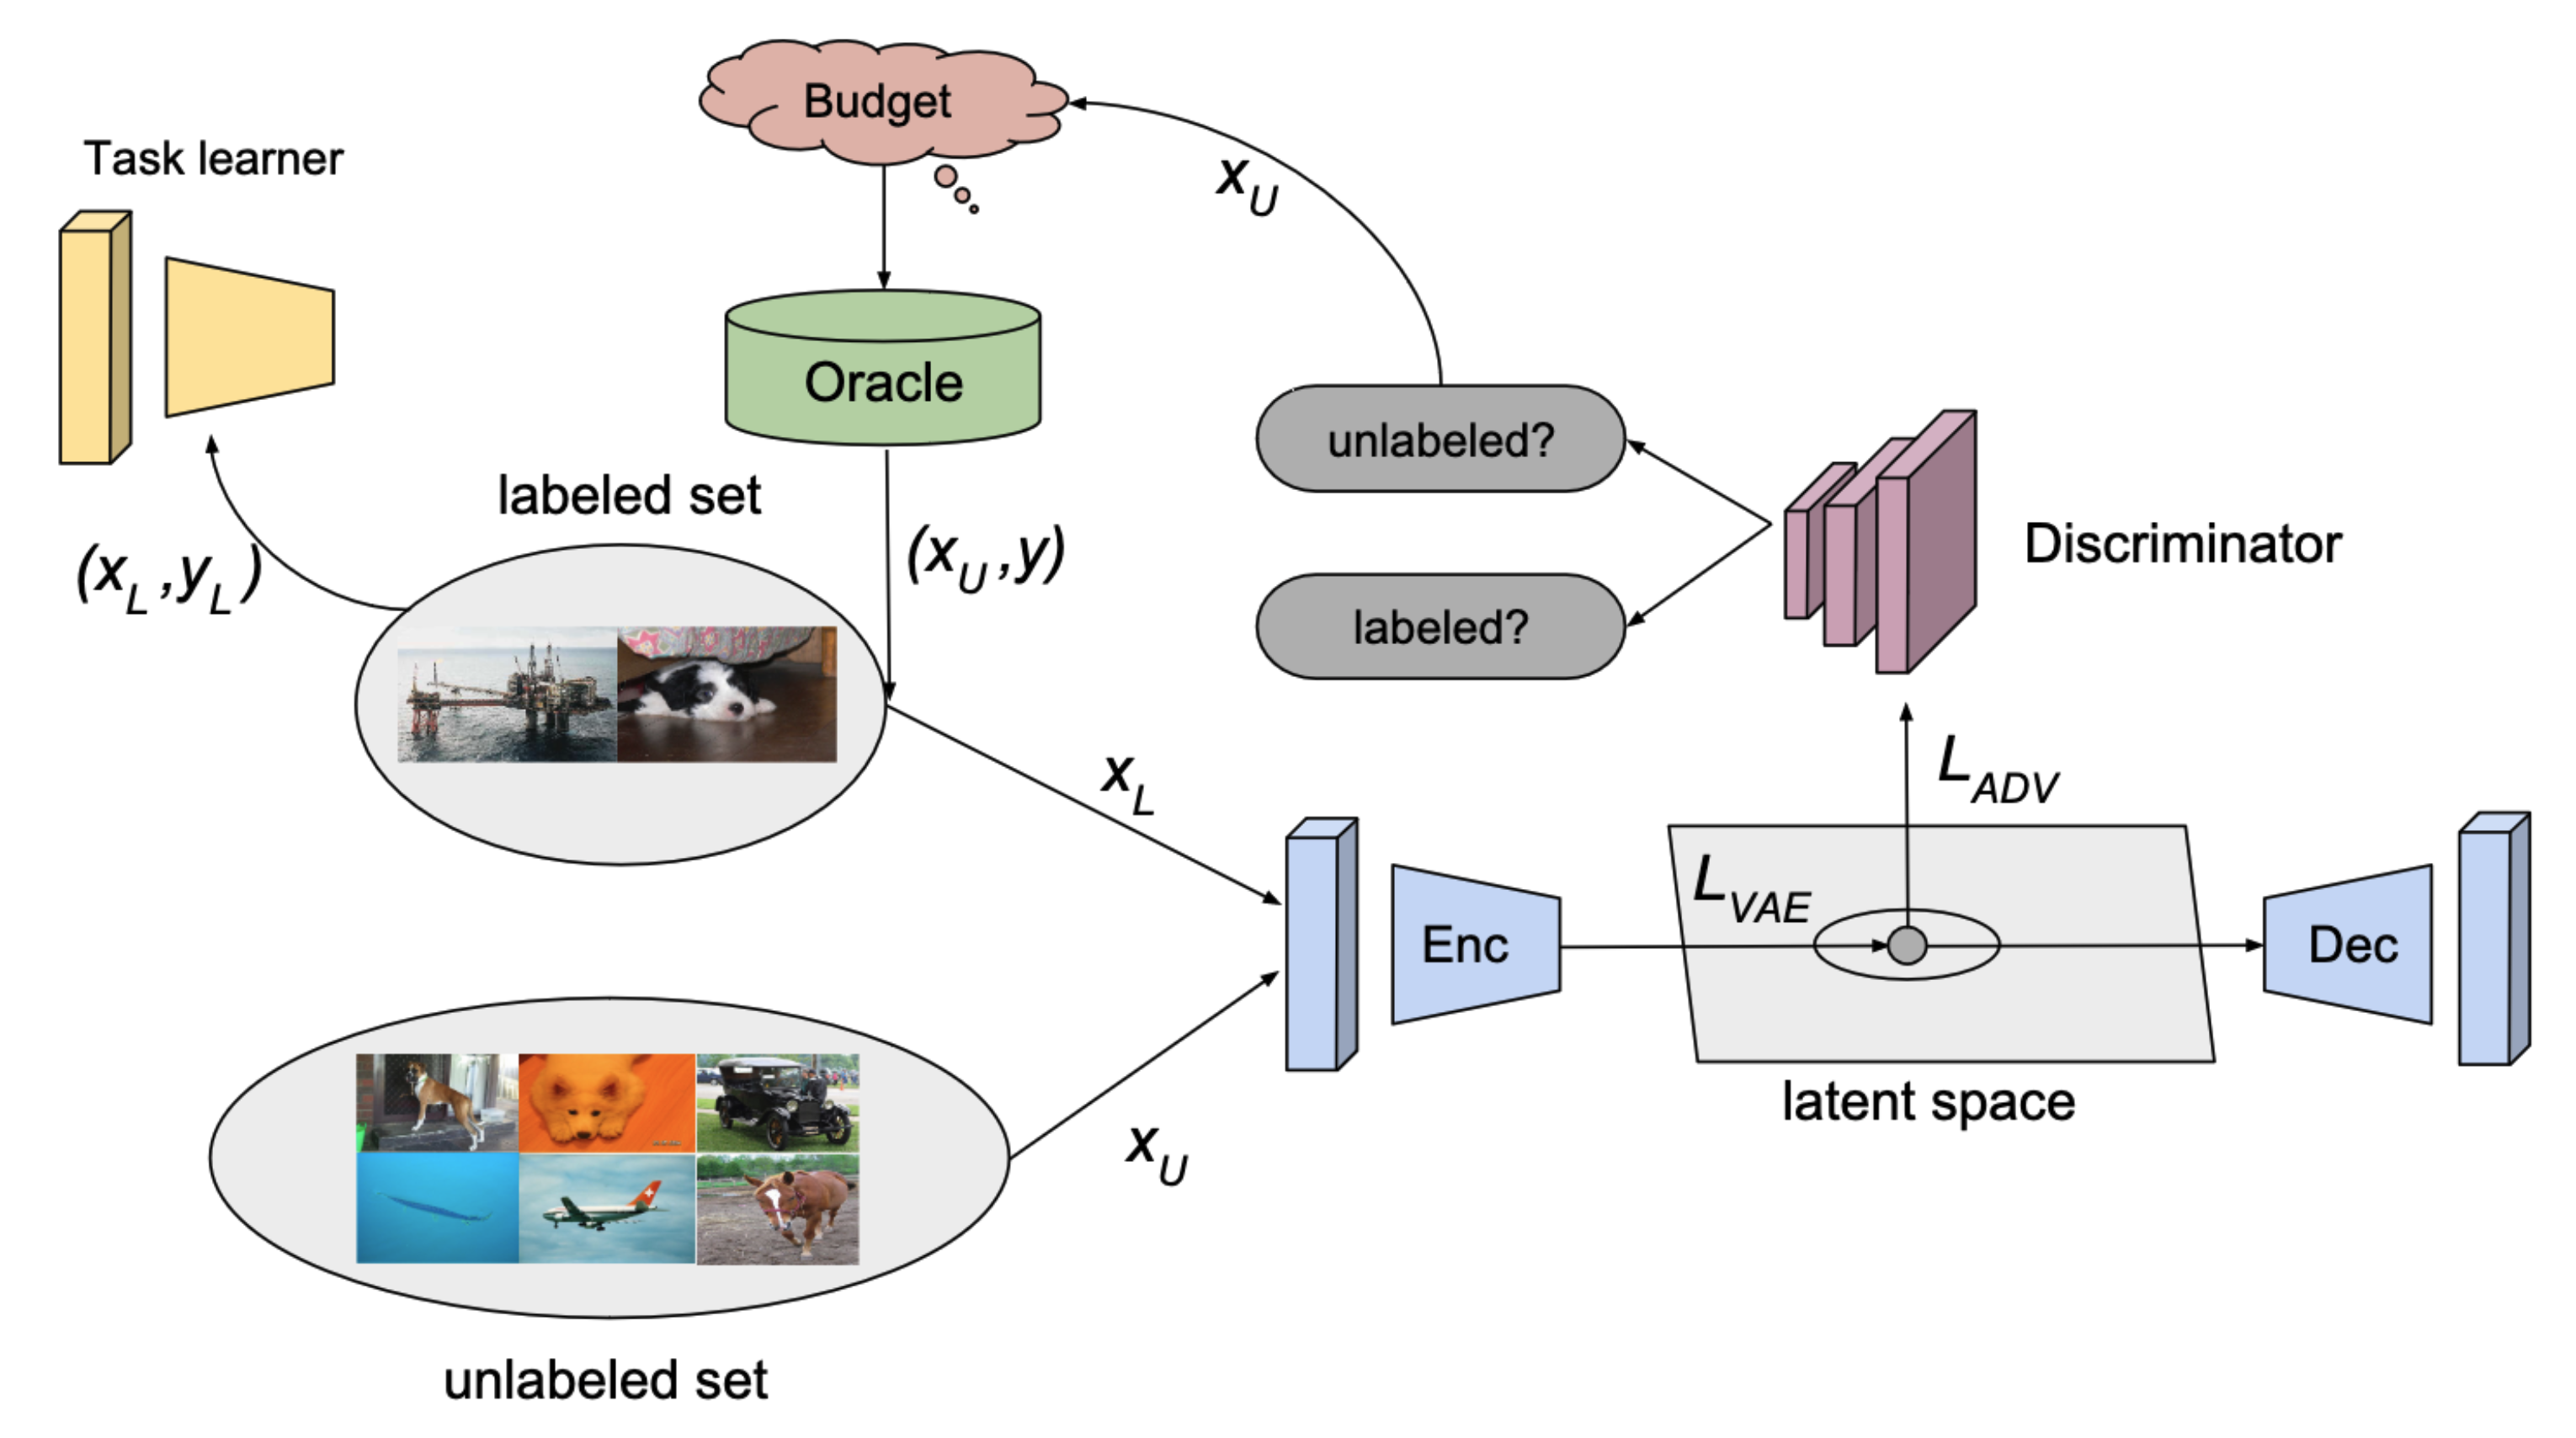
\includegraphics[width=.8\linewidth]{images/Vaal_idea.png}
    \caption[Visualization of \gls{vaal}]{Illustration of the idea of \gls{vaal} taken from the paper of Sinha et al. \cite{sinha2019variational}.}
    \label{fig:VAAL}
\end{figure}


\section{Continual Learning}
\label{sec:Related_work:Continual_Learning}
In this section, we will present the continual learning algorithms used in our experiments. These are elastic weight
consolidation (\gls{ewc}) \cite{kirkpatrick2017overcoming}, memory aware synapses (\gls{mas}), asymmetric loss approximation by single-side overestimation
(\gls{alasso}), incremental moment matching (\gls{imm}) and averaged gradient episodic memory (\gls{a-gem}) \cite{lopez2017gradient}. While we aim to give
a detailed explanation of these approaches, we refer to the original papers for any further details. \par

\subsection{Elastic Weight Consolidation}
\label{sec:Related_work:Continual_Learning:EWC}
Elastic weight consolidation (\gls{ewc}) \cite{kirkpatrick2017overcoming} is a structural regularization approach proposed by Kirkpatrick et al.
\gls{ewc} was the first approach aiming to overcome catastrophic forgetting by regularizing model parameters. This is done by adding a regularization
term to the loss function, which resembles $l_2$ regularization. The regularization loss is introduced to constrain important parameters for
task $N-1$ to stay close to their previous values when training on task $N$. To come up with an importance measure for the parameters,
Kirkpatrick et al. view neural network training from a probabilistic perspective, modeling the weight distribution using the Bayes rule:
\begin{equation}
    p(\theta \mid D) = \frac{p(D \mid \theta) \cdot p(\theta)}{p(D)}.
\end{equation}
When applying the logarithm, this can be rewritten as
\begin{equation}
    \log p(\theta \mid D) = \log p(D \mid \theta) + \log p(\theta) - \log p(D)
\end{equation}
and when splitting the whole dataset $D$ into $D_{1:N-1}$ and $D_N$, this equates to
\begin{equation}
    \log p(\theta \mid D) = \log p(D_N \mid \theta) + \log p(\theta \mid D_{1:N-1}) - \log p(D_N),
\end{equation}
meaning that only the term $\log p(\theta \mid D_{1:N-1})$ is dependent on the previous tasks. Therefore, it must contain the full information 
about all previous tasks. Since $\log p(\theta \mid D_{1:N-1})$ cannot be computed, Kirkpatrick et al. approximate it using Laplace's approximation
\cite{mackay2003information}, obtaining a Gaussian distribution with mean of $\theta^*_{1:N-1}$ and covariance matrix $[\mathbb{I}_{D_{1:N-1}}]^{-1}$,
where
\begin{equation}
    \mathbb{I}_{D_{1:N-1}} = \mathbb{E} [- \frac{\partial^2 \theta (\log (p(\theta \mid D_{1:N-1})))}{\partial^2 \theta} \mid_{\theta^*_{D_{1:N-1}}}]
\end{equation} 
which is the Fisher information matrix (\gls{fim}) as shown by Aich \cite{aich2021elastic}. A large value of $F_i$, the $i$-th diagonal of the \gls{fim},
indicates a small variance in the posterior distribution of the parameter, meaning that it is important for previous tasks. Therefore, $F_i$, is used as an
importance measure for the $i$-th parameter. To conclude, the loss function for a Task $N$ is altered to
\begin{equation}
    \mathcal{L}(\theta) = \mathcal{L}_B(\theta) + \sum_i \frac{\lambda}{2} F_i \cdot (\theta_i - \theta^*_{N-1,i})^2,
\end{equation}
where $\mathcal{L}_B(\theta)$ is the loss function of the model on the current task (e.g. cross-entropy loss), $\theta_i$ is the $i$-th parameter of the model,
and $\theta^*_{N-1,i}$ is the $i$-th parameter of the model trained on the previous task. The hyperparameter $\lambda$ is used to trade-off between
learning new tasks and retaining knowledge of previous tasks.

\subsection{Memory Aware Synapses}
\label{sec:Related_work:Continual_Learning:MAS}
Memory aware synapses (\gls{mas}), like \gls{ewc}, is a structural regularization method proposed by Aljundi et al. \cite{aljundi2018memory}. 
In line with \gls{ewc}, \gls{mas} aims to prevent catastrophic forgetting by regularizing model parameters. The main difference between \gls{ewc} and
\gls{mas} the composition of their importance measure. While \gls{ewc} relies on Fisher information to compute parameter importances, \gls{mas} uses
gradient magnitude to estimate the importance of a parameter for previous tasks. To derive the importance measure, the authors first observe that the
effect of small changes to the network parameters on the prediction can be approximated as follows
\begin{equation}
    f(x_k; \theta + \delta) - f(x_k; \theta) \approx = \sum_i g_i(x_k) \cdot \delta_i
\end{equation}
where $g_i(x_k) = \frac{\partial(f(x_k;\theta))}{\partial \theta_i}$  is the gradient with respect to parameter $\theta_i$ when evaluating the model at
input $x_k$. Since most classification models, like neural networks, for example, have a multi-dimensional output Aljundi et al. propose to use the gradient
of the squared $l_2$ norm in this setting, i.e. $g_i(x_k) =  \frac{\partial[l^2_2(f(x_k;\theta))]}{\partial \theta_i}$. With the approximation given by the
equation above, the authors claim that the importance of a parameter $\theta_i$ can be computed as
\begin{equation}
    \omega_i = \frac{1}{n} \sum_{k=1}^n \lVert g_i(x_k) \rVert
\end{equation}
where $n$ is the number of data points observed so far. The advantage of computing the importance measure as stated above is that it can be updated when-
ever a new data point is observed. However, it is more efficient to update the $\omega$s batch-wise. The overall loss function for a task $N$ is
then altered for the standard setting as follows
\begin{equation}
    \mathcal{L}(\theta) = \mathcal{L}_N(\theta) + \lambda \sum_i \omega_i \cdot (\theta_i - \theta^*_{N-1,i})^2
\end{equation}
where $\lambda$ again is the hyperparameter used to trade-off between learning new tasks and retaining the knowledge of previous tasks.

\subsection{Asymmetric Loss Approximation by Single-Side Overestimation}
\label{sec:Related_work:Continual_Learning:ALASSO}
Asymmetric loss approximation by single-side overestimation (\gls{alasso}) is a structural regularization method proposed by Park et al. \cite{park2019continual}.
\gls{alasso} is an extension of \gls{si} proposed by Zenke et al. \cite{zenke2017continual}. Park et al. claim that \gls{alasso} \enquote{mitigates the limitations of SI}.
The main observation they made about \gls{si} is that it underestimates the true loss on the unobserved side of the loss
function because it assumes that the loss function is symmetric. Park et al. first show that this assumption is not always correct through empirical observation
and then present a new approach to approximate the loss function on the unobserved side. We present the fundamental observation and idea of \gls{alasso} in figure
\ref{fig:Alasso}. Since \gls{alasso} extends the \gls{si} framework, we strongly recommend the reader familiarize themselves with \gls{si} before
trying to understand \gls{alasso}. In the following, we will assume that the reader is familiar with \gls{si} and only explain the extension that \gls{alasso}
brings to \gls{si}. \par
Since \gls{alasso} is a structural regularization method like \gls{mas} and \gls{ewc}, it alters the loss function as follows
% Total loss equation
\begin{equation}
    \tilde{\mathcal{L}}^N = \mathcal{L}^N + c \sum_k \mathcal{L}_s^{N-1}(\theta_k,a),
\end{equation}
meaning that it adds a surrogate loss to the loss function, which is controlled via the hyperparameter $c$. To understand how the surrogate loss is composed
\gls{alasso} first introduces $\alpha(\theta_k)$, which determines for a model parameter if it is on the observed or unobserved side of the loss function.
$\alpha(\theta_k)$ is defined as follows
% Alpha equation
\begin{equation}
    \alpha(\theta_k) = (\theta_k - \hat{\theta}^N_k) (\hat{\theta}^{N-1}_k - \hat{\theta}^N_k)
\end{equation}
The surrogate loss $\mathcal{L}^N_s(\theta_k,a)$ is then defined as follows
% Loss estimation equation
\begin{equation}
    \mathcal{L}_s^n(\theta_k,a) = \begin{cases} \hat{\Omega}^N_k (\theta_k - \hat{\theta}_k)^2 & \text{if} \alpha(\theta_k) > 0 \\
    (a \hat{\Omega}^N_k + \epsilon)(\theta_k - \hat{\theta}_k)^2 & \text{if} \alpha(\theta_k) \leq 0 \end{cases}.
\end{equation}
Again, the variable $a (>1)$ is a hyperparameter used to control the amount of overestimation if the parameter is on the unobserved side of the loss function.
The constant $\epsilon$ is used to make sure that the loss on the unobserved side is always overestimated, i.e., $(a \hat{\Omega}^N_k + \epsilon) > \hat{\Omega}^N_k$.
The second contribution of \gls{alasso} is its derivation of the optimal coefficient $\hat{\Omega}^N_k$ for the approximation of the loss function on the \textit{observed}
side. According to Park et al., $\hat{\Omega}^N_k$ is determined by the following equation
% Omega equation
\begin{equation} \label{eq:ALASSO_Omega}
    \hat{\Omega}^N_k = \frac{\omega^N_k + \omega^{1:N-1}_k}{(\hat{\theta}^N_k - \hat{\theta}^{N-1}_k)^2},
\end{equation}
where $\omega^N_k$ and $\omega^{1:N-1}_k$ are given by
% Small Omega equation
\begin{gather} \label{eq:ALASSO_Small_Omega}
    \omega^N_k = \mathcal{L}^N(\hat{\theta}^{N-1}_k) - \mathcal{L}^N(\hat{\theta}^N_k) \\
    \omega^{1:N-1}_k = -c\mathcal{L}^{N-1}_s(\hat{\theta}^N_k,a)
\end{gather}
Because of the ambiguous influence of the hyperparameters $c$ and $a$ to the approximation of the loss function, the authors of \gls{alasso} propose to decouple them. More
precisely, they suggest using $c'$ and $a'$ instead of $c$ and $a$ in equation 3.23.

\begin{figure} [ht]
    \centering
    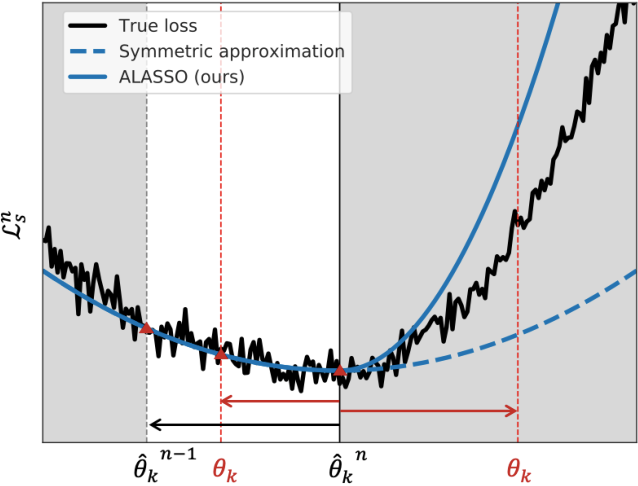
\includegraphics[width=.5\linewidth]{images/Alasso_Idea.png}
    \caption[Visualization of \gls{alasso}]{Illustration of the idea of \gls{alasso} taken from the paper of Park et al. \cite{park2019continual}. The authors of \gls{alasso}
     state that, \gls{si}
    underestimates the unobserved side of the loss function and hence a better approximation of the loss function is achieved by overestimating it.}
    \label{fig:Alasso}
\end{figure}

\subsection{Incremental Moment Matching}
\label{sec:Related_work:Continual_Learning:IMM}
Incremental moment matching (\gls{imm}) is a structural regularization approach, proposed by Lee et al. \cite{lee2017overcoming}.
\gls{imm} deviates from approaches like \gls{mas} and \gls{ewc} in that it should not be viewed as a single method but rather a framework of multiple methods,
many of which can be combined. The main idea of \gls{imm} is to match the first and second moments of the posterior distribution $p(\theta \mid D_{1:N})$ of the model 
parameters given all tasks up to the current one. As in \gls{ewc}, the posterior distribution cannot be computed. Therefore, it is approximated via a Gaussian distribution which
we call $q_{1:N}$. The first approach to matching these moments is called mean-based incremental moment matching, also known as mean-\gls{imm}. The weight
update of mean-\gls{imm} is the analytical solution of the problem to minimize the weighted sum of \gls{kl} divergences between each $q_i$ and $q_{1:N}$
\cite{goldberger2004hierarchical}, i.e. the solution to
\begin{equation}
    \argmin_{\mu^*_{1:N},\Sigma^*_{1:N}} \sum_{i=N-k}^N \alpha_i \cdot KL(q_i \mid \mid q_{1:N})
\end{equation}
which is given by
\begin{gather}
    \mu^*_{1:N} = \sum_{i=N-k}^N \alpha_i \cdot \mu_i \\
    \Sigma^*_{1:N} = \sum_{i=N-k}^N \alpha_i (\Sigma_i + (\mu_i - \mu^*_{1:N})(\mu_i - \mu^*_{1:N})^T)
\end{gather}
The $\alpha_i$ are the mixing coefficients that weigh the previous $k$ tasks and have the constraint $\sum_{i=N-k}^N \alpha_i = 1$.  \\
The second approach to matching the moments is called mode-based incremental moment matching, also known as mode-\gls{imm}. mode-\gls{imm}
further incorporates covariance information from previous tasks to match the first and second moments of the posterior distribution. 
The mean and covariance update for mode-\gls{imm} is given by
\begin{gather}
    \mu^*_{1:N} = \sum_{i=N-k}^N \alpha_i \cdot (\sum_{i=N-k}^N \alpha_i \Sigma_i^{-1} \mu_i) \\
    \Sigma^*_{1:N} = (\sum_{i=N-k}^N \alpha_i  \Sigma_i^{-1})^{-1}
\end{gather}
To approximate the covariance matrix, mode-\gls{imm} uses the inverse of the \gls{fim} like \gls{ewc}. Furthermore, the authors assume that
the model parameters are pairwise independent, making the covariance matrix diagonal and therefore save computation. \par
Apart from moment matching methods, \gls{imm} also includes approaches to transfer model parameters from previous tasks. The first approach is called
weight transfer. When using continual learning with weight transfer, the parameters of the previous task are used as initialization for the
current task. This approach is very similar to the term warm start commonly used in active learning. $l_2$-transfer, which is a special form of 
$l_2$ regularization, is the next transfer technique. $l_2$-transfer can be seen as a special form of \gls{ewc} where all the $F_i$s are set to 1. 
With $l_2$-transfer, the loss function is altered to
\begin{equation}
    \log p(y_N \mid X_N, \mu_N) - \lambda \cdot {\lVert \mu_N - \mu_{N-1} \rVert}^2_2
\end{equation}
with $\lambda$ being a hyperparameter. The third transfer technique is \textbf{Drop-transfer}. Drop-transfer
\begin{equation}
    \hat{\mu}_{N,i} = \begin{cases} \mu_{N,i}, & \text{if the }i \text{th node is turned off} \\
    \frac{1}{1-p} \cdot \mu_{N,i} - \frac{p}{1-p} \cdot \mu_{N-1,i}, & \text{otherwise}  \end{cases}
\end{equation}
where $p$ is the dropout ratio. Drop-transfer can be seen as a further regularizer for continual learning, with similar effect to $l_2$-transfer albeit
being orthogonal to it. In algorithm \ref{alg:IMM}, we show the pseudocode for \gls{imm} with weight-transfer and $l_2$-transfer. \par

\begin{algorithm}
    \caption{\gls{imm} with weight-transfer, $l_2$-transfer} \label{alg:IMM}
    \begin{algorithmic}
        \Require data $f\{ (X_1,Y_1),\ldots,(X_N,Y_N)\}$, balancing hyperparameter $\alpha$ with $\sum_{i=1}^k \alpha_i = 1$,
        regularization hyperparameter $\lambda$
        \return $w_{1:N}$
        \State $w_0 \leftarrow $ InitializeNN()
        \For{$i=1:N$}
            \State $w_{i*} \leftarrow w_{i-1}$
            \State Train($w_{i*},X_i,Y_i$) with $L(w_{i*},X_i,Y_i) + \lambda \cdot (\lVert w_{i*} - w_{i-1} \rVert)^2_2$
            \State $m=\max (0,i-k)$
            \If{type is mean-IMM}
            \State $w_{i*} \leftarrow \sum_{t=max(0,i-k)}^i \alpha_t w_{t}$
            \ElsIf{type is mode-IMM}
            \State $F_{i*} \leftarrow$ CalculateFisherMatrix($w_{i*},X_i,Y_i$)
            \State $\Sigma_{1:i} \leftarrow (\sum_{t=max(0,i-k)}^i \alpha_t F_{t*} w_{t*})^{-1}$
            \State $w_{i*} \leftarrow \Sigma_{1:i} \cdot (\sum_{t=max(0,i-k)}^i \alpha_t F_{t*} w_{t*})$
            \EndIf
        \EndFor
    \end{algorithmic}
\end{algorithm}

\subsection{Averaged Gradient Episodic Memory}
\label{sec:Related_work:Continual_Learning:AGEM}
Averaged gradient episodic memory (\gls{a-gem}) is an exemplar rehearsal approach to continual learning, proposed by Chaudhry et al. \cite{chaudhry2018efficient}.
\gls{a-gem} is based on gradient episodic memory (\gls{gem}) \cite{lopez2017gradient}, aiming to make it more efficient than \gls{gem} while maintaining similar or
even better performance. We recommend reading the original paper for a more detailed explanation of \gls{gem}. \par
Like \gls{gem}, \gls{a-gem} uses a so-called episodic memory $M$ for all previous tasks $M_k (k<N)$. \gls{a-gem} aims to avoid catastrophic forgetting by ensuring
that the average loss for the previous tasks does not increase while simultaneously aiming to minimize the loss on the current task. Formally, \gls{a-gem} proposes
a solution to the following objective 
\begin{equation}
    \text{minimize}_\theta \hspace{0.2cm} \mathcal{L}(f_\theta,T_N) \text{ s.t. } \mathcal{L}(f_\theta,T) \leq l(f_\theta^{N-1},T) \text{ where } T = \bigcup_{i<N} T_i
\end{equation}
where $f_\theta^{N-1}$ is the model trained for the previous task. The optimization problem for this objective is given as
\begin{equation}
    \text{minimize}_{\tilde{g}} \hspace{0.2cm} \frac{1}{2} {\lVert g - \tilde{g} \rVert}^2_2 \text{ s.t. } \tilde{g}^T g_{ref} \geq 0 \forall k < N
\end{equation}
where $g_{ref}$ is a gradient computed by randomly sampling from the episodic memory of all past tasks. The optimization problem has the solution 
\begin{equation}
    \tilde{g} = g - \frac{g^T g_{ref}}{g^T_{ref} g_{ref}} g_{ref}
\end{equation}
which is the gradient update used by \gls{a-gem}. \par
When running \gls{a-gem}, we need to decide on two hyperparameters: The first one is $S$, the number of samples from the episodic memory $M$ to compute $g_{ref}$. The second
one is $P$, the number of patterns (or data points) stored in the episodic memory after each task.


\section{Model Stealing}
\label{sec:Related_work:Model_Stealing}
In this section, we will present related work from the model stealing domain. This consists of ActiveThief \cite{pal2020activethief}, a model stealing framework using
active learning.

\subsection{ActiveThief}
\label{sec:Related_work:Model_Stealing:ActiveThief}
ActiveThief is a novel model stealing approach proposed by Pal et al. \cite{pal2020activethief}. Inspired by prior theoretical \cite{chandrasekaran2020exploring}
and practical work \cite{shi2018active}, they use active learning to choose which samples to query the target model. Using active learning in the model stealing
domain provides three major benefits: First, it makes it easier for the attacker to create a thief dataset. Data is abundant nowadays, whereas labeling large amounts
of data remains a time-intensive task. By using active learning, which works on unlabeled data, creating a thief dataset is sped up immensely.
Second, active learning aims to query the most informative samples, yielding the most performant model with as little data as possible. Third, by using samples selected
by active learning to query the target model, the model stealing attack can successfully be disguised as a benign query process. Pal et al. demonstrate this by showing 
that ActiveThief successfully evades \gls{prada} \cite{juuti2019prada}, a state-of-the-art model stealing defense which detects attacks by analyzing the distribution of distances
between queries. \par
The authors of ActiveThief evaluate their framework using the active learning strategies Random, Uncertainty \cite{lewis1995sequential}, CoreSet \cite{sener2017active},
DeepFool-based active learning (\gls{dfal}) \cite{ducoffe2018adversarial} and a custom combination of \gls{dfal} and CoreSet. They use a custom \gls{cnn} architecture
for both the target and substitute model and show that ActiveThief can successfully steal the target model for multiple benchmark datasets such as MNIST and CIFAR-10.
A visualization of the model stealing workflow proposed by Pal et al. is shown in figure \ref{fig:ActiveThief}.

\begin{figure} [ht]
    \centering
    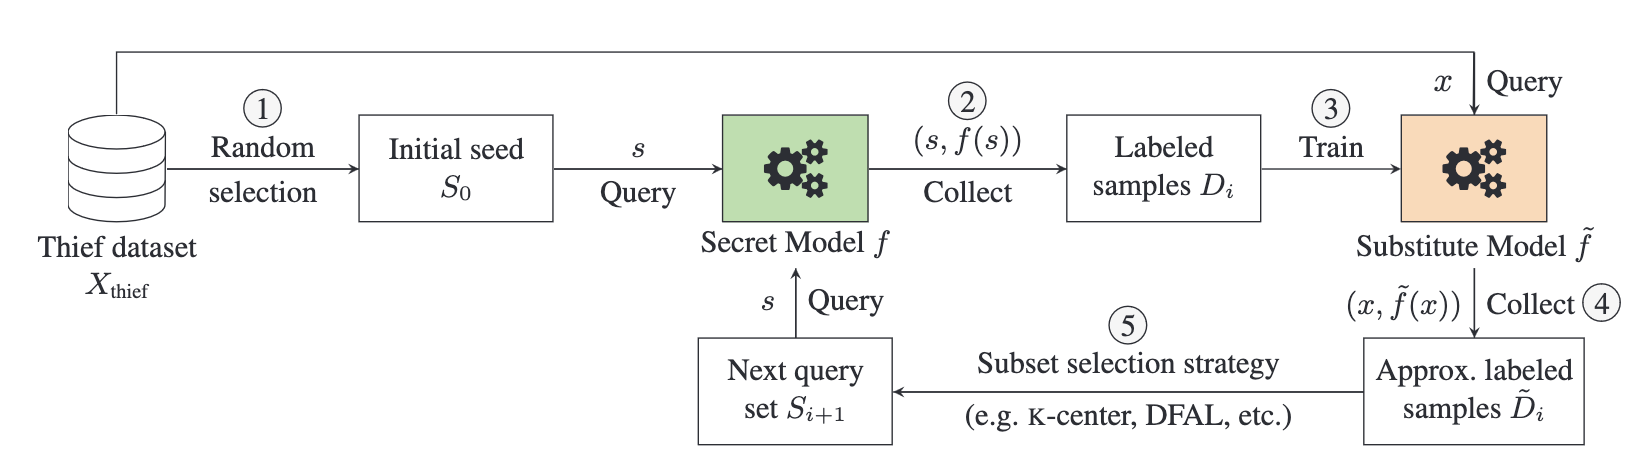
\includegraphics[width=.9\linewidth]{images/ActiveThief_Idea.png}
    \caption[Visualization of ActiveThief]{Illustration of the model stealing workflow proposed by \cite{pal2020activethief}. Inspired by
    \cite{chandrasekaran2020exploring}, Pal et al. use Active Learning to select the next samples to query the target model.}
    \label{fig:ActiveThief}
\end{figure}

%% ---------------------
%% | / Example content |
%% ---------------------